\tikzset{every picture/.style={line width=0.75pt}} %set default line width to 0.75pt        

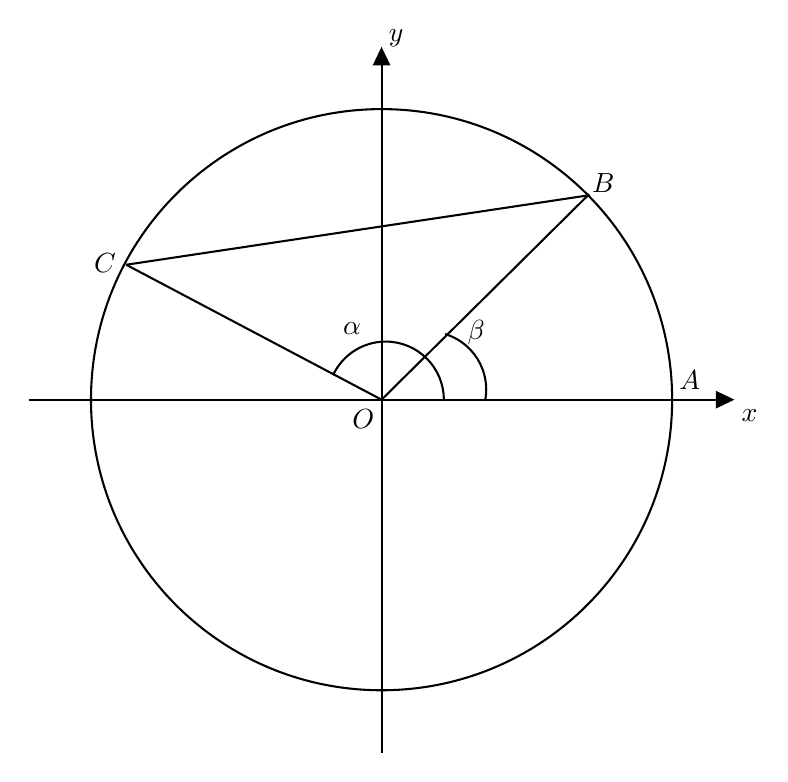
\begin{tikzpicture}[x=0.75pt,y=0.75pt,yscale=-1,xscale=1]
%uncomment if require: \path (0,371); %set diagram left start at 0, and has height of 371

%Shape: Circle [id:dp09037269014980676] 
\draw   (190,180) .. controls (190,102.68) and (252.68,40) .. (330,40) .. controls (407.32,40) and (470,102.68) .. (470,180) .. controls (470,257.32) and (407.32,320) .. (330,320) .. controls (252.68,320) and (190,257.32) .. (190,180) -- cycle ;
%Straight Lines [id:da38997271294485203] 
\draw  (160,180) -- (497,180); % eixo x
\draw [shift={(500,180)}, rotate = 180] [fill={rgb, 255:red, 0; green, 0; blue, 0 }  ][line width=0.08]  [draw opacity=0] (8.93,-4.29) -- (0,0) -- (8.93,4.29) -- cycle    ;
%Straight Lines [id:da5041518340149789] 
\draw    (330,350) -- (330,13); % eixo y
\draw [shift={(330,10)}, rotate = 450] [fill={rgb, 255:red, 0; green, 0; blue, 0 }  ][line width=0.08]  [draw opacity=0] (8.93,-4.29) -- (0,0) -- (8.93,4.29) -- cycle    ;
%Straight Lines [id:da8860425225499272] 
\draw    (330,180) -- (207,115); % segundo quadrante
%Straight Lines [id:da5369351916234646] 
\draw    (330,180) -- (430,81); % primeiro quadrante
%Shape: Arc [id:dp9919207634955951] 
\draw  [draw opacity=0] (336.37,150.68) .. controls (341.29,151.74) and (345.76,154.01) .. (349.46,157.16) -- (330,180) -- cycle;

\draw (360,180) arc (0:-155:28); % alfa
\draw (380,180) arc (10:-73:28); % beta

\draw    (206.9,115) -- (430,81.5); % segmento superior


% Text Node
\draw (328,183.4) node [anchor=north east] [inner sep=0.75pt]    {$O$};
% Text Node
\draw (472,176.6) node [anchor=south west] [inner sep=0.75pt]    {$A$};
% Text Node
\draw (430,81.5) node [anchor=south west] [inner sep=0.75pt]    {$B$};
% Text Node
\draw (310,150) node [anchor=south west] [inner sep=0.75pt]   {$\alpha $};
% Text Node
\draw (370,155) node [anchor=south west] [inner sep=0.75pt]  {$\beta $};
% Text Node
\draw (502,183.4) node [anchor=north west][inner sep=0.75pt]    {$x$};
% Text Node
\draw (332,11.6) node [anchor=south west] [inner sep=0.75pt]    {$y$};
% Text Node
\draw (190,120) node [anchor=south west] [inner sep=0.75pt]    {$C$};

\end{tikzpicture}